%%%%%%%%%%%%%%%%%%%%%%%%%%%%%%%%%%%%%%%%%%%%%%%%%%%
%
%  New template code for TAMU Theses and Dissertations starting Fall 2016.  
%
%
%  Author: Sean Zachary Roberson
%  Version 3.17.09
%  Last Updated: 9/21/2017
%
%%%%%%%%%%%%%%%%%%%%%%%%%%%%%%%%%%%%%%%%%%%%%%%%%%%
%%%%%%%%%%%%%%%%%%%%%%%%%%%%%%%%%%%%%%%%%%%%%%%%%%%%%%%%%%%%%%%%%%%%%%
%%                           SECTION IV
%%%%%%%%%%%%%%%%%%%%%%%%%%%%%%%%%%%%%%%%%%%%%%%%%%%%%%%%%%%%%%%%%%%%%



\chapter{EVENT RECONSTRUCTION \label{cha:eventreco}}
In the CMS detector, collisions happen in a small longitudinal region near the center called the luminous region or interaction region. Collisions themselves are not recorded, only the particles that get created. The origin of one or more new particles is called a vertex. An event is the set of particle measurements in the detector associated to a single beam-beam crossing. It is the job of the reconstruction software to process the raw information and identify physics objects for a given event.

 \begin{figure}[H]
 	\centering
 	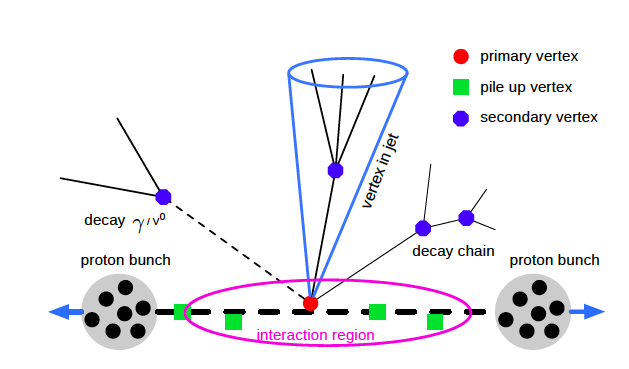
\includegraphics[width=0.75\textwidth]{figures/eventvertex.png}
 	\singlespace
 	\caption{Schematic diagram for an event at the LHC.}
 	\label{fig:vertex}
 \end{figure}

Recall from the previous section that events are filtered online by so-called trigger systems, so that only interesting events are written to disk. The collision triggering the readout is called the primary vertex, while other collisions from the beams are called pile-up. Secondary vertices refer to the other production points, when particles are created from decay or hard-scattering. This is shown in Figure \ref{fig:vertex}. Particles from the primary vertex usually have a high transverse momentum ($p_{T}$), making them interesting and easier to study.



\section{Tracks and Vertices}
\label{sec:track}

 Trajectories of charged particles, or tracks, are reconstructed from the position hits in the detector. From the collection of tracks in an event, the primary and any secondary vertices are reconstructed.

 The first step of the reconstruction process is referred to as local reconstruction and it consists of the clustering of \textit{zero-suppressed} signals above specified thresholds in pixel and strip channels into hits. The next step is track reconstruction, which refers to the process of using the reconstructed hits to obtain estimates for the momentum and position parameters of the charged particles responsible for the detector hits. 

 The tracking software at CMS\cite{TRK-11-001} is commonly referred to as the combinatorial Track Finder (CTF), which is an adaptation of the combinatorial Kalman Filter \cite{Billoir:1989mh},\cite{BILLOIR1990219},\cite{Mankel:1997dy}, which in turn is an extension of the Kalman filter\cite{Fruhwirth:1987fm} to allow pattern recognition and track fitting to occur in the same framework. The collection of reconstructed tracks is produced by multiple passes or iterations of the same CTF track reconstruction sequence, in a process called iterative tracking. 

The basic idea of iterative tracking is that the initial iteration seach for tracks that are easiest to find (e.g., of relatively large $p_{T}$, and produced near the interaction region). After each iteration, hits associated with tracks are removed, thereby reducing the combinatorial complexity, and simplifying subsequent iterations in a seach for more difficult classes of tracks (e.g., low $p_{T}$, or greatly displaced tracks).

Each iteration proceeds in four steps:

\begin{itemize}
	\item Seed generation which provides track candidates consisting of a few (2 or 3) hits. Seeds are generated in the innermost layers of the tracker and are commonly reffered to as "proto-tracks".
	\item Track finding, which is based on a Kalman filter. It extrapolates the seed trajectories along the expected flight path of a charged particle, searching for additional hits that can be assigned to the track candidate.
	\item Track fitting. A module that is used to provide the best possible estimate of the parameters of each trajectory by means of a Kalman filter.
	\item Track selection. This step sets the quality flags and discards tracks that fails certain specified criteria.
\end{itemize}

Each iteration is configured for different purposes and the tunable parameters for seed generation and final track selection selected accordingly. For example, during the 2011 run, six iterations were applied. Iteration 0 was designed for prompt tracks (originating near the pp interaction point) that have three pixel hits. Iteration 1 was used to recover prompt tracks that have only two pixel hits. Iteration 2 was configured to find low-$p_{T}$ prompt tracks and iterations 3-5 were intended to recover tracks not found in the previous iterations.

Note that the tracks reconstruction process described above produces the main track collection used by the CMS collaboration. However, variants of this software are also used for more specialized purposes such as electron track reconstruction or HLT track reconstruction.

The next step in the reconstruction process utilizes the available reconstructed tracks to measure the location (and its associated uncertainty) of all proton-proton interaction vertices in each event. This includes the "signal" vertex and any vertices from pileup collisions. Primary-vertex reconstruction\cite{Speer:927395} consists of three steps:

\begin{itemize}
	\item Selection of the tracks,
	\item Clustering of the tracks that appear to originate from the same interaction vertex, and
	\item Fitting for the position of each vertex using its associated tracks.
\end{itemize}

Track selection involves choosing tracks consistent with being produced promptly in the primary interaction region by imposing requirements on the number of strip and pixel hits associated with a track, the normalized $\chi^{2}$ from a fit to the trajectory, and the maximum value of significance of the transverse impact parameter relative to the centre of the LHC beamspot. The beamspot represents a 3D profile of the luminous region, where the LHC beams collide in the CMS detector.

 The selected tracks are clustered on the basis of their $z$-coordinates at their point of closest approach to the center of the beam spot by using a \textit{deterministic annealing} (DA)\cite{726788} algorithm. The DA algorithm finds the global minimum for a problem with many degrees of freedom, in a way that is analogous to that of a physical system approaching a state of minimal energy through a series of gradual temperature reductions.

After identifying candidate vertices based on the DA clustering in \textit{z}, those candidates containing at least two tracks are then fitted using an \textit{adaptive vertex fitter}\cite{Fruhwirth:1027031} to compute the best estimate of vertex parameters, including its $x$, $y$, and $z$ position and covariance matrix, as well as the indicators for the success of the fit, suach as the number of degrees of fredom for the vertex, and weights of the tracks used in the vertex.

\section{Particle Flow}

As mentioned in Section 2, CMS is one of the two general-purpose detectors at the LHC, and as such, it was designed based on the concept of cylindrical detection layers, as we can see in Figure \ref{fig:cmsslice}.

 \begin{figure}[h]
  	\label{fig:cmsslice}
 	\centering
 	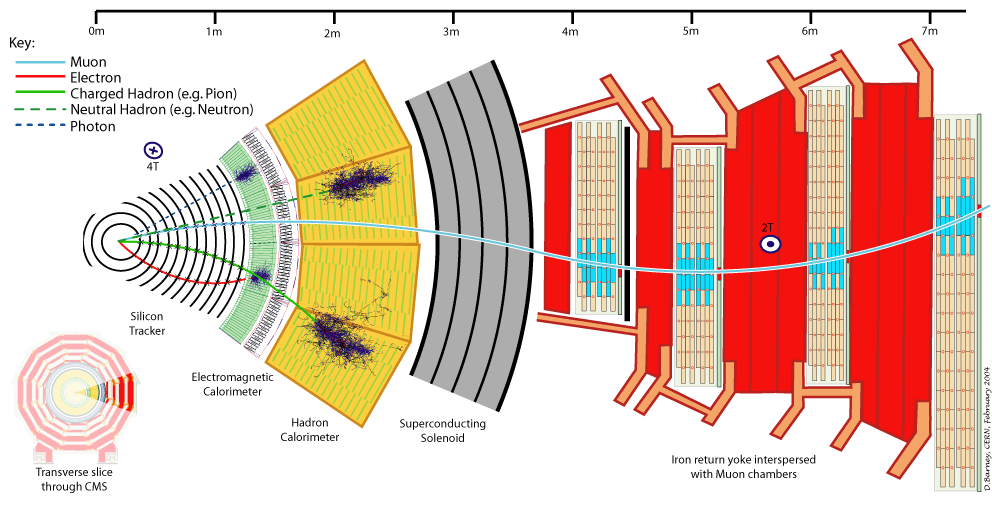
\includegraphics[width=0.75\textwidth]{figures/image005.gif}
 	\singlespace
 	\caption{Cross-sectional view of the CMS detector with all of the sub-detectors labeled. The colored lines correspond to different particle types. Each particle interacts with different pieces of the detector and may or may not be bent by the magnetic field. Reprinted from \cite{CMSSlice}}
 \end{figure}

An optimal event description can be achieved by correlating the basic elements from all detector layers (tracks and clusters) to identify each final-state particle, and by combining the corresponding measurements to reconstruct the particle properties on the basis of this identification. At CMS, this approached is called \textit{particle-flow (PF) reconstruction}.

The reconstructed and identified individual particle list includes muons, electrons, photons, charged hadrons, as well as stable and unstable neutral hadrons. These particles can be non-isolated, and even originate from an intricate overlap of reconstructed charged particles, ECAL and HCAL energy clusters, and signals in the muon chambers.

Referring back to Figure \ref{fig:cmsslice}, photons and neutral hadrons are in general identified by ECAL and HCAL clusters with no track link. No attempt is made to distinguish the various species of neutral and charged hadrons in the PF reconstruction. Electrons can be identified by a track and an ECAL cluster, with a momentum-to-energy ratio compatible with unity, and not connected to an HCAL cluster. Finally, muons and neutrinos would traverse the calorimeters with little or no interactions. While neutrinos would escape undetected, muons would be identified by a track in the inner tracker connected to a track in the muon detectors.

The PF concept was developed and used for the first time by the ALEPH experiment at LEP\cite{BUSKULIC1995481} and can now be used in hadron colliders due to the very fine spatial granularity of the detectors. In particular, CMS is very well suited for PF reconstruction due to its highly-segmented tracker,  a fine-grained ECAL, and an hermetic HCAL.

% A given particle is, in general, expected to give rise to serveral PF elements in the various CMS subdetectors. The reconstruction of a particle therefore first proceeds with a link algorithm that connects PF elements from different subdetectors. The probability for the algorithm to link elements from one particle inly is limited by the granularity of the various subdetectors and by the number of particles to resolve per unit of solid angle. The probability to link all elements of a given particle is mostly limited by the amount of material encountered upstream of the calorimeters and the muon detector, which might lead to trajectory kinks and to creation of secondary particles. 

 \begin{figure}[h]
  	\label{fig:pf}
 	\centering
 	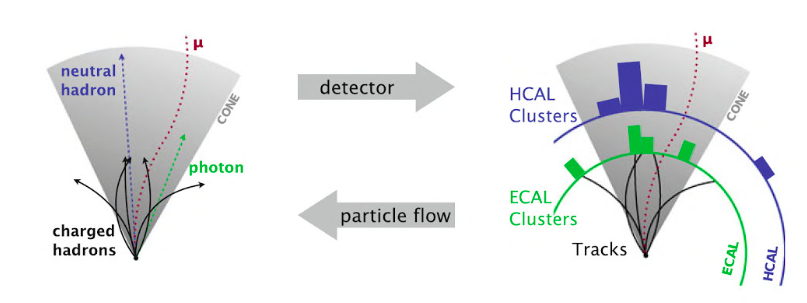
\includegraphics[width=0.75\textwidth]{figures/jets.png}
 	\singlespace
 	\caption{CMS Particle Flow algorithm. The diagram shows how collisions lead to particle decays and final state particles. On the right side of the diagram the tracks and deposits in the CMS detector are shown. The left side shows that PF candidates are derived from detector information and then become inpur for the PF algorithm that uses them to construct high-level physics objects like electrons, which are then used by analysts to reconstruct the collision event. Reprinted from \cite{CMS-PAS-PFT-09-001}}
 \end{figure}

\section{Jets}

\section{b-tagging}

\section{Event Generation}

\section{Detector Simulation}

